% \PassOptionsToPackage{unicode}{hyperref}
% \PassOptionsToPackage{naturalnames}{hyperref}
\documentclass[12pt, aspectratio=169]{beamer}
\usetheme[progressbar=frametitle]{metropolis}
\usepackage[utf8]{inputenc}
\usepackage[T1]{fontenc}
% \usetheme{Arguelles}
\usepackage{textpos}
\usepackage{amsmath,amsthm,amsfonts}
\usepackage[hyperref=true,style=numeric-comp,uniquename=init,doi=false,url=false,backend=biber,maxnames=2]{biblatex}
\DeclareNameAlias{sortname}{given-family}
\usepackage[utf8]{inputenc}

\usepackage{tikz}
\usetikzlibrary{shapes.geometric, arrows, positioning}
\tikzstyle{startstop} = [rectangle, rounded corners, minimum width=3cm, minimum height=1cm, text centered, draw=black, fill=red!30]
\tikzstyle{details} = [rectangle, minimum height=1cm, align=center, draw=black, fill=green!30]
\tikzstyle{io} = [rectangle, rounded corners, align=center, draw=black, fill=blue!20]
\tikzstyle{process} = [rectangle, minimum width=3cm, minimum height=1cm, align=center, draw=black, fill=orange!30]
\tikzstyle{decision} = [diamond, minimum width=3cm, minimum height=1cm, align=center, draw=black, fill=green!30]
\tikzstyle{arrow} = [thick,->,>=stealth]


\setbeamertemplate{footline}[page number]{}

\addbibresource{bibliography.bib}
% \addtobeamertemplate{frametitle}{}{%
% 	\begin{textblock*}{\textwidth}(12.5cm, -0.65cm)
% 		\includegraphics[width=0.1\textwidth]{CUNY_Logo.png}~
% 		\includegraphics[width=0.05\textwidth]{NSF_4-Color_bitmap_Logo.png}
% 	\end{textblock*}}
\title{Structural Identifiability in Julia: A Tutorial}
\institute{\inst{1}Graduate Center, CUNY}
\author[Ilia Ilmer]{Ilia Ilmer\inst{1}}
\date{March 23, 2022}
\begin{document}
\maketitle
\begin{frame}{Outline}
    \begin{itemize}
        \item Introduction
        \item {\tt StructuralIdentifiability.jl}
        \item {\tt SIAN.jl}
        \item Examples
        \item Conclusions
    \end{itemize}
\end{frame}
\begin{frame}{Introduction}
    \begin{itemize}
        \item Structural identifiability is a theoretical notion\pause{}: ``Can one determine parameters of a given ODE model (assuming noiseless outputs and sufficiently strong inputs)?''\pause{}
        \item {\it Global} identifiability means we can determine the value of parameter(s) uniquely\pause{}
        \item {\it Local} identifiability means we can determine up to multiple values
    \end{itemize}
\end{frame}
\begin{frame}{Example}
    \begin{equation}
        \begin{cases}
            \dot{x} = A^2x + b, \\
            y = x
        \end{cases}
    \end{equation}
    \pause{}
    Solution: \begin{itemize}
        \item \(x(0), b\) are globally identifiable, \(A\) is identifiable only locally according to {\tt SIAN.jl}.\pause{}
        \item \(b\) is globally identifiable, \(A\) is locally identifiable according to {\tt StructuralIdentifiability.jl}. Note that there is no information about \(x\).
    \end{itemize}

\end{frame}
\begin{frame}{{\tt SIAN.jl}\footfullcite{hong_global_2020}}
    \begin{columns}
        \column{0.5\textwidth}
        \begin{center}
            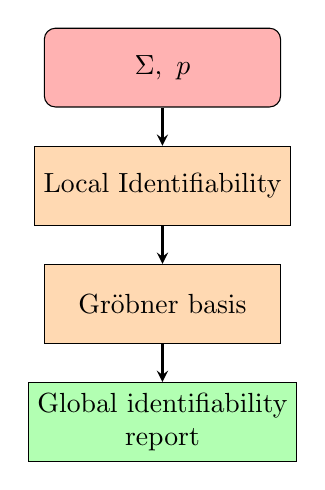
\begin{tikzpicture}[node distance=1.5cm]
                \node (input) [startstop] {\(\Sigma,~p\)};
                % \node (maxsys) [process, below of=input] {maximal system of\\algebraic equations};
                \node (truncate) [process, below of=input] {Local Identifiability};
                \node (determine) [process, below of=truncate] {Gr\"obner basis};
                \node (output) [details, below of=determine] {Global identifiability\\report};

                \draw [arrow] (input) -- (truncate);
                % \draw [arrow] (maxsys) -- (truncate);
                \draw [arrow] (truncate) -- (determine);
                \draw [arrow] (determine) -- (output);
            \end{tikzpicture}
        \end{center}
        \column{0.5\textwidth}
        \begin{itemize}
            \item SIAN is a Monte-Carlo algorithm.
            \item Input: ODE model with outputs \(\Sigma\), probability of correctness \(p\).
            \item Local identifiability is determined via identifiability rank condition.
            \item Global identifiability is analyzed via Gr\"obner basis.
        \end{itemize}
    \end{columns}
\end{frame}
\begin{frame}{{\tt StructuralIdentifiability.jl}\footfullcite{dong2022differential}}
    \begin{columns}
        \column{0.7\textwidth}
        \begin{itemize}
            \item Input: ODE model with outputs \(\Sigma\), probability of correctness \(p\).
            \item Local identifiability is based on Sedoglavic's algorithm \cite{sedoglavic2002probabilistic}.
            \item Global identifiability is determined via field of coefficients of input-output equations
            \item Can differentiate Single- or Multi-experiment identifiability
        \end{itemize}
        \column{0.3\textwidth}
        \begin{center}
            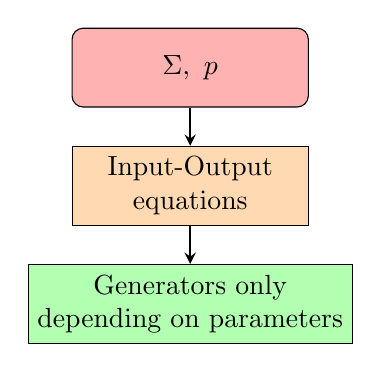
\begin{tikzpicture}[node distance=1.5cm]
                \node (input) [startstop] {\(\Sigma,~p\)};
                \node (ioeq) [process, below of=input] {Input-Output\\equations};
                \node (gen) [details, below of=ioeq] {Generators only\\depending on parameters};
                \draw [arrow] (input) -- (ioeq);
                \draw [arrow] (ioeq) -- (gen);
            \end{tikzpicture}
        \end{center}

        %     \begin{tikzpicture}[node distance=1.5cm]
        %         \node (ioeq) [details, xshift=-8cm] {Input-Output\\equations};
        %         \node (wronsk) [details, right of=ioeq, xshift=1.5cm] {Compute\\Wronskians};
        %         \node (rref) [details, right of=wronsk,xshift=1.5cm] {Compute bound\\and coefficient\\via rank};
        %         \node (gen) [details, right of=rref,xshift=2.5cm] {Out: bound, generators};

        %         \draw [arrow] (ioeq) -- (wronsk);
        %         \draw [arrow] (wronsk) -- (rref);
        %         \draw [arrow] (rref) -- (gen);
        %     \end{tikzpicture}
    \end{columns}

\end{frame}
\begin{frame}{Examples}

\end{frame}
\begin{frame}{Conclusions and Summary}
    \begin{itemize}
        \item Parameter identifiability can be solved in Julia Language from 2 different perspectives
        \item No one-size-fits-all solution
        \item Future work includes mutliple enhancements to ODE preprocessing, Gr\"obner basis computation, integration with more SciML packages
    \end{itemize}
\end{frame}
\printbibliography{}
\end{document}